% !TEX root = /Users/saxer/Documents/uppsalaDV/pkd/project/Cashier-System/Report.tex
% !TEX encoding = UTF-8 Unicode
\documentclass[11pt]{article}
\usepackage[a4paper,top=3cm,bottom=2cm,left=3cm,right=3cm,marginparwidth=1.75cm]{geometry}
\usepackage[T1]{fontenc}
\usepackage[utf8]{inputenc}
\usepackage[english]{babel}
\usepackage{graphicx}
\usepackage{listings}
\usepackage{color}

\lstset{
  frame=none,
  xleftmargin=2pt,
  stepnumber=1,
  numbers=left,
  numbersep=5pt,
  numberstyle=\ttfamily\tiny\color[gray]{0.3},
  belowcaptionskip=\bigskipamount,
  captionpos=b,
  escapeinside={*'}{'*},
  language=haskell,
  tabsize=2,
  emphstyle={\bf},
  commentstyle=\it,
  stringstyle=\mdseries\rmfamily,
  showspaces=false,
  keywordstyle=\bfseries\rmfamily,
  columns=flexible,
  basicstyle=\small\sffamily,
  showstringspaces=false,
  morecomment=[l]\%,
}

\begin{document}
\title{Project - Business register and database}
\author{Group 23: Jesper Saxer, Sebastian Lhådö , Grim Moström}
\date{\today}
\maketitle{}
\newpage
\section{Introduction}
Conducting business on a professional level can be overwhelming without the proper tools and systems. It is essential that business actions and cash flows are tracked. Without  a functional system it can be complicated to trace how eventual mistakes or disadvantageous business actions are affecting the business and even worse, to track inventories and cash flows during the declaration of taxes. A proper business tool such as a Business register can be helpful to administrate multiple users in the business in order to keep track of actions and cash flows.
This project aims to create a complete system that keeps track of stock, purchases, identification of users and most importantly the in and outgoing cash flows. In addition it aims to provide a customer based cart system in order to assist the customer, improving the user experience, guiding the customer in the decision and payment process.\\\\
The project was conducted during a limited time span, which in some aspects has hasted the process, affecting the product. The project resulted in a complete business system with the desired functions. However, some flaws are included, such as limited test cases. The general quality of the product is correlating to the project goals, but a more vast timespan had improved the visual interaction and more test cases.\\\\
The project has contributed well to the learning of functional programming and use of functions. Even some aspects of visual programming has been learnt. Thus, giving increased experience of both front- and backend program development.
\newpage
\tableofcontents
\newpage
\section{Illustration of the Business system}
In order to deliver a complete understanding of the business system, we have chosen to map our system in graphical context. This way we can guide the reader through the build of the system and it’s hidden functions.
\\
The following graphical illustration is a brief summary of the main files of the business system.
\subsection{Flow chart}
\begin{figure}[h]
  \includegraphics[width=\linewidth]{FlowChart.png}
  \caption{Flow chart over the shop}
  \label{fig:flow chart}
\end{figure}
\newpage
\section{Branch declarations}
\subsection{Database}
The database administrates and stores the main functions. Through the database we can store the inventory, create users, and receive purchases or changes in stock.
The database is functioning as an information bank in which information can be edited such that it fits the needs of the administrator, thus correlating to the reality of the business process in practice. Without the database, it is impossible to store the flow of information that is added into the system. This implies that it is an essential piece of the complete business system.
\\
Please read further in Branch \& Data structure specification X:X for further information
\subsection{User}
When registering business-transactions it is important for the system to determine whether the user is an administrator, employee or a customer in order to offer the right services and properties.
The system is designed such that it offers an administrator the full access to change all variables in the system, including the users available to administer the system.
A customer on the other hand only has access to information needed to purchase goods, eg. stock, price and products.
\\\\
Please read further in Branch \& Data structure specification X:X for further information
\subsection{Item}
One of the most essential parts of the business system is the Item specification. The items may be changed or modified as the stock or price changes. Further you upload one of these changes to the database in order to update price and inventory. An item holds all the information needed to specify the products values, such as the stock, EAN code, price, and name.
\\\\
Please read further in Branch \& Data structure specification X:X for further information
\subsection{Cart}
The cart is a temporary list of chosen products by the User.  This cart holds products in order to sum up the list of chosen products and giving the user an overview of its choices. From here it is easy to navigate in order to add more products or remove them. This way the usability of the system increases since the customer can iterate the shopping list while being able to keep on shopping.\\\\
Please read further in Branch \& Data structure specification X:X for further information\\
\subsection{Interface}
\subsubsection{Functional Interface}
The interface is divided in two levels of functionality. The function interface, and the graphical menu.
Interface functions is our gathering channel from our systems flow chart. This is the channel in which the User interacts with the complete business system. By hiding all help functions in the back end systems you can easily communicate in a front-end manor to the user, simplifying the systems usability, improving the user experience. This way we enable the customer to handle the system without any further practical guidance than what is offered by the business system itself and its users guide.
\\\\
Please read further in Branch \& Data structure specification X:X for further information
\subsubsection{Graphical Interface}
The graphical interface is a visualization of the interface functions to get the complete front-end product. With a graphical interface the User is further being guided in the useage of the system. This is the final level of the product, surfacing to the interaction with the User.
\\\\
Please read further in Branch \& Data structure specification specification X:X for further information.
\newpage
\section{Branch \& Data structure specification}
\subsection{Database}
Database.hs is the way we choose to represent a Database in our Cashier-System. Our Database.hs has its own data types which is defined the following preset:
\begin{lstlisting}
type Id = Int -- Ean for item, userId for users
type Database a = [(a,Id)]
\end{lstlisting}

The identity of a user is defined by a User code, based on integers. These numbers are unique for each User and makes  it easy to identify two different users with similar names.
The identity of Items are identified by a matching EAN code, scanned on the products back. This serial code defines the sort of product and is unique for the specific type of product specified.
\\
The data type Database a = [(a,Id)]  is polymorphic. This implicates that it is non type specific.  This way, Database can hold both user identities and items. This is fitting to the needs of information storage to be held in the business system. In summarization the Database takes one polymorphic argument and returns a tuple containing a product, or user together with an ID.
\\\\
The following functions are reachable if Database.hs is imported
\begin{lstlisting}
empty :: Database a
deleteWithID :: Id -> Database a -> Database a
delete :: Eq a => a -> Database a -> Database a
insert :: a -> Id -> Database a -> Database a
grab :: Eq a => a -> Database a -> a
grabWithID :: Id -> Database a -> a
\end{lstlisting}

Notation: In the structure of the function specifications for the functions above. You can see a collection of types with an arrow pointing right. The value presented after the last arrow indicates what the complete function returns. The other arrows is separating arguments that the function takes while being called.
\\\\
The same fundamental constructional frame of functions is maintained through the whole project. For specified code, please read attached file.

\newpage
\subsection{User}
User.hs is the representation of User identities in the Cashier-System. Our User.hs has its own data structure which is defined in the following way.
\begin{lstlisting}
type Name = String
type Id = Int
type Wallet = Int
type Spent = Int
type IsAdmin = Bool

data User = User Name Id Wallet Spent IsAdmin deriving (Show, Eq)
\end{lstlisting}
Every User takes the following arguments:
Name is represented by a string of characters bound between two “ ” symbols.
Example: “Name”
Id is represented by a series of numbers, identifying the user by unique numerical identification by integers.
Example: Id = 1234
Wallet: The Wallet is a data type representing the amount of money a user have stored in the system. This virtual money represented by integers is later at disposal on the products put into the system.
Spent represents the amount of money a user have spent in our system. The purpose of this data type is to track cash flows in the system and follow up on the system revenues.
IsAdmin keeps tracks the user itself have admin properties or not. This is very important in order to keep the business systems integrity level. By having administrator properties, the system disables customers access to sensitive data and essential product maintenance functions.
\\\\
The following functions are reachable if User.hs is imported\\
\begin{lstlisting}
newUser       :: Name   -> Id   -> Wallet -> Spent -> IsAdmin -> User
setName       :: Name   -> User -> User
getName       :: User   -> Name
setId         :: Id     -> User -> User
getId         :: User   -> Id
fillWallet    :: Wallet -> User -> User
removeWallet  :: Wallet -> User -> User
removeSpent   :: User   -> User
makeAdmin     :: User   -> User
removeAdmin   :: User   -> User
getAdminStatus :: User -> Bool
addSpent      :: Spent  -> User -> User
reduceSpent :: Spent -> User -> User
removeSpent :: User -> User
getWallet     :: User   -> Wallet
clearWallet   :: User   -> User
\end{lstlisting}
These data types are all related to preset functions explained in previous section.
The data types are all enabling changes in the main data type of its kind.
\subsection{item}
Item.hs is the way we chose to represent a product of in the Cashier-System. Our Item.hs has its own data structure which is defined in the following way.
\begin{lstlisting}
type Name  = String
type Ean   = Int
type Price = Int
type Stock = Int
data Item = Item Name Ean Price Stock deriving (Show,Eq)
\end{lstlisting}
This means that every item has the following Arguments.\\
Name, the name in the form of a string.\\
Ean, the barcode that is on the item itself.\\
Price, the price we want to take for the item.\\
Stock, the amount of items we have in storage.\\
The following functions is reachable if Item.hs is imported.\\
\begin{lstlisting}
createItem :: Name -> Ean -> Price -> Stock -> Item
setName :: Name   -> Item -> Item
getName         :: Item   -> Name
setEan          :: Ean    -> Item -> Item
getEan          :: Item   -> Ean
setPrice        :: Price  -> Item -> Item
getPrice        :: Item   -> Price
addToStock      :: Stock  -> Item -> Item
removeFromStock :: Stock  -> Item -> Item
replaceStock :: Stock -> Item -> Item
getStock        :: Item   -> Stock
\end{lstlisting}
An example would be setName "Coca-Cola" (Item "cola" 1234 10 0) -> (Item "Cola-Cola" 1234 10 0)\\
Here you can see that setName is being called with two arguments, first a Name and secondly an Item and with these two arguments it returns a new Item. For specified code, please read attached file.
\subsection{Cart}
In order to enable customers to interact and store their product choices in the system, we have created the branch Cart. Cart.hs imports both Item.hs and Database.hs which is stated through the flowchart.\\
Cart has only one data type which is declared in the following way:\\
\begin{lstlisting}
type Cart = [Item]
\end{lstlisting}
The data type Cart is put the linked list of items. This is to create a simple structure where we can easily get an overview of chosen products.\\
Cart.hs is imported and makes the following functions reachable.\\
\begin{lstlisting}
empty :: Cart
addToCart :: Item -> Cart -> Cart
removeFromCart :: Item -> Cart -> Cart
calculatePrice :: Cart -> Int
getFirst :: Cart -> (Item,Cart)
cartUpdate :: Item -> Cart -> Cart
\end{lstlisting}
All functions specified aims to make Cart edible for Users. The names of functions are relatively self explanatory. As mentioned in previous branch and data specifications, the types put in are contained among the first arrows, whilst the last output is specified last in each function. For specified code, please read attached file.
\subsection{Interface}
\subsubsection{Functional Interface}
The functional interface is the systems most advanced branch as it collects and handles all other branches as a root of the system.Interface.hs handles all branches and is imported and called through different functions. To make it more readable we have added headings in order to understand the different specifications. For specified code, please read attached file.
\begin{lstlisting}
imports
import Item
import User
import Cart
import Database
import Test.HUnit
\end{lstlisting}
As mentioned, you can see that all branches are imported into the functional interface. One addition to this is our automated tests conducted through test.Hunit.
To read more about debugging and testing, please read chapter about testing and debugging. For specified code, please read attached file.
\begin{lstlisting}
Data types

type Name     = String
type Ean      = Int
type Price    = Int
type Stock    = Int
type Id       = Int
type Wallet   = Int
type Spent    = Int
type IsAdmin  = Bool
data Interface = Interface User (Database User) (Database Item) Cart deriving (Show,Eq)
\end{lstlisting}
Many of these data types are mentioned previously and are relatively self explanatory in its context. They are empirically needed to be restated to increase readability of code. Each branch specifies data types used in the program. This way the usability and quality of the system increases significantly for future edits. For specified code, please read attached file.\\
\begin{lstlisting}
Interface
newInterface :: User -> Database User -> Database Item -> Cart -> Interface
\end{lstlisting}
new interface specifies what types the interface takes in the system. The system is as you can see built of the other branches, calling user, databases, cart and creates the interface. For specified code, please read attached file.
\begin{lstlisting}
getDatabaseItem :: Interface -> Database Item
getDatabaseUser :: Interface -> Database User
\end{lstlisting}
The interface returns the databases it holds. For specified code, please read attached file.
\begin{lstlisting}
User administration
getUser :: Interface -> User
createUser :: Name -> Id -> Wallet -> Spent -> IsAdmin -> Interface -> Interface
removeUser :: User -> Interface -> Interface
findUser :: Id -> Interface -> User
\end{lstlisting}
The user administration calls all the functions needed to handle users from the User branch. This way the interface simplifies the user administration as it is gathered and called with simple functions. For specified code, please read attached file.
\begin{lstlisting}
setUserName :: Name -> User -> Interface -> Interface
getUserName :: User -> Name
setUserId :: Id -> User -> Interface -> Interface
getUserAdmin :: Interface -> Bool
makeUserAdmin:: User -> Interface -> Interface
removeUserAdmin:: User -> Interface -> Interface
\end{lstlisting}
\begin{lstlisting}
Item administration
findItem :: Ean -> Interface -> Item
createItem :: Name -> Ean -> Price -> Stock -> Interface -> Interface
removeItem :: Item -> Interface -> Interface
\end{lstlisting}
The item administration calls all the functions needed to handle items from the Item branch. This way the interface simplifies the user administration as it is gathered and called with simple functions. For specified code, please read attached file.
\begin{lstlisting}
setUserName :: Name -> User -> Interface -> Interface
getUserName :: User -> Name
setUserId :: Id -> User -> Interface -> Interface
getUserAdmin :: Interface -> Bool
makeUserAdmin:: User -> Interface -> Interface
removeUserAdmin:: User -> Interface -> Interface
\end{lstlisting}
setItemName :: Name -> Item -> Interface -> Interface
getItemEan :: Item -> Ean
setItemEan :: Ean -> Item -> Interface -> Interface
setItemPrice :: Price -> Item -> Interface -> Interface
\begin{lstlisting}
Wallet
getWallet :: User -> Interface -> Wallet
fillWallet :: Int -> User -> Interface -> Interface
reduceWallet :: Int -> User -> Interface -> Interface
clearWallet :: User -> Interface -> Interface
\end{lstlisting}
The interface calls all wallet functions that is needed to adjust or create wallet values. For specified code, please read attached file.
\begin{lstlisting}
stock handling
addToStock :: Int -> Item -> Interface -> Interface
removeFromStock :: Int -> Item -> Interface -> Interface
replaceStock :: Int -> Item -> Interface -> Interface
\end{lstlisting}
The interface calls all stock functions that is needed to adjust or create stock values. For specified code, please read attached file.
\begin{lstlisting}
Cart Handling
addToCart :: Item -> Interface -> Interface
removeFromCart :: Item -> Interface -> Interface
buy :: Interface -> Interface
calculateCartPrice :: Interface -> Price
getCart :: Interface -> Cart
\end{lstlisting}
The interface calls all cart functions that is needed to adjust or create temporary cart values.
\subsubsection{Graphical interface}
The graphical interface file Menu.hs withholds all information regarding the terminal actions that the user is interacting with to purchase products. This implicates that our following Users guide will mainly be concerning this file. To make a functional menu system we have had to make some additional imports to the file:
\begin{lstlisting}
import Interface
import System.Process
\end{lstlisting}
The functional interface file is imported in order to make its content implemented in the user interface menu. Its code is rather large but its usability is quite simple. System.Process is imported as a standard help function in order to be able to clear the terminal and increasing its usability.
\\
To understand the graphical interface, please read User guide and attached file.
\newpage
\section{User guide}
Welcome to this quick start User's Guide of the Business System Interface. Since the User can be both an Administrator and Customer, we have chose to make external guides for these different properties.
\subsection{User functions}
This system requires that you have a terminal and that you can open it. When you have located your terminal you want to find the directory where the folder Cashier-System is stored in our case it’s stored in:
\begin{lstlisting}
/Users/your_directory/Cashier-System
\end{lstlisting}
 therefore to locate it in the terminal we have to write:
\begin{lstlisting}
 cd your_directory/Cashier-System/
\end{lstlisting}
You should now have your terminal looking something like this:
\\
\begin{figure}[h]
  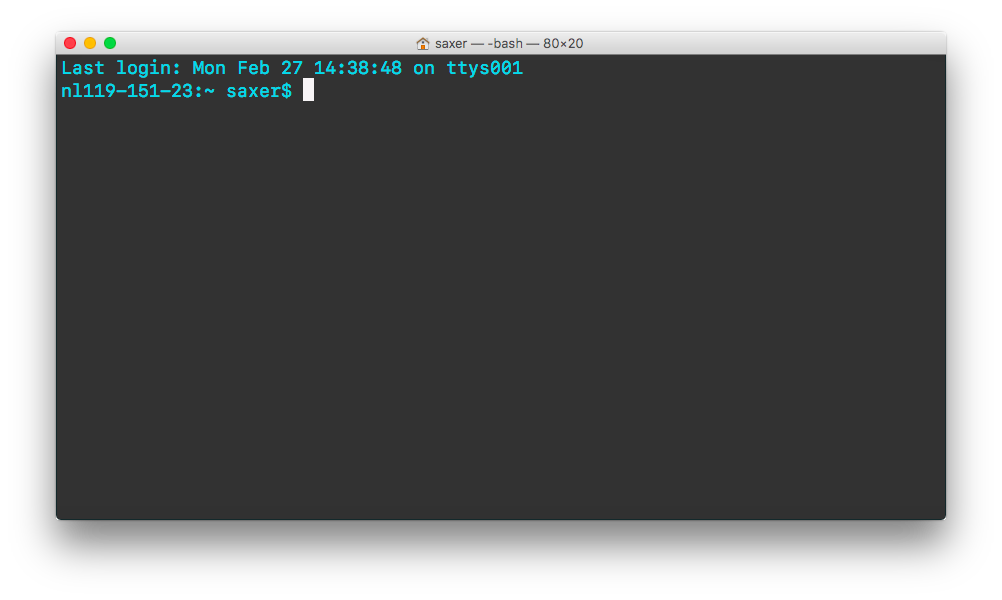
\includegraphics[width=\linewidth]{interface1.png}
  \caption{Terminal}
  \label{fig:Terminal}
\end{figure}
\\
\newpage
The next step is to type in ghci and load the file menu.hs and now we’re ready to shop! The code should look like this :\\
ghci [enter]\\
>:l menu.hs [enter]\\
Since the code compiled we proceed by typing in: main.\\\\
What you should be seeing now is the interface for the shop. This page is the front of the business system that ties all functions and code together. From here you’ll need to know how to navigate and explore the shop and all its functions. Your terminal window should now be looking like this:
\\
\begin{figure}[h]
  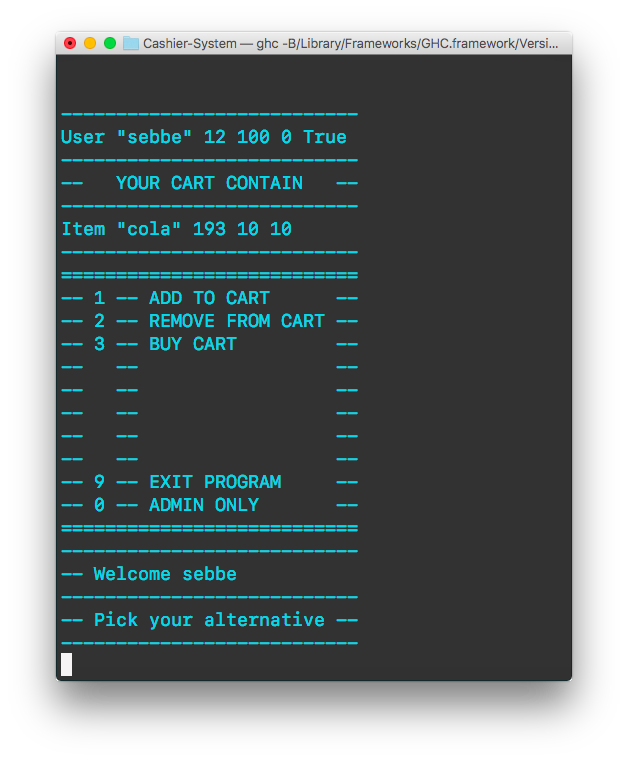
\includegraphics[width= 250px]{interface2.png}
  \caption{cart}
\end{figure}
\newpage
At the top of the interface the current user status is displayed. The user is represented as the previously mentioned data type data User = User Name Id Wallet Spent IsAdmin.
Thus, returning all current values implemented on the users account.\\
The second section of the interface is the current cart for the user.\\
This section contains stored goods that you add to cart whilst shopping.\\
The third section is the menu representing the different alternatives the user has available. Each choice is presented in numerical alternatives.\\
The fourth section is where the messages will be shown, for example a greeting, or a warning that a invalid number has been applied.\\
The fifth and last section is where the user writes commands for the menu to work i.e if the user wants to add a product to its cart and browse what the shop has to offer we type in a “1” and press enter. If we want to purchase the content of the current cart we press “4” and hit enter. As you can see the menu is a command based platform, interacting with the customer by presenting available choices, waiting for a User response.\\\\
\subsubsection{Adding or removing an item to cart}
If we want to add an item to the cart we start by navigate to the “add to cart” by typing 1 and hit enter.
\\
\begin{figure}[h!]
  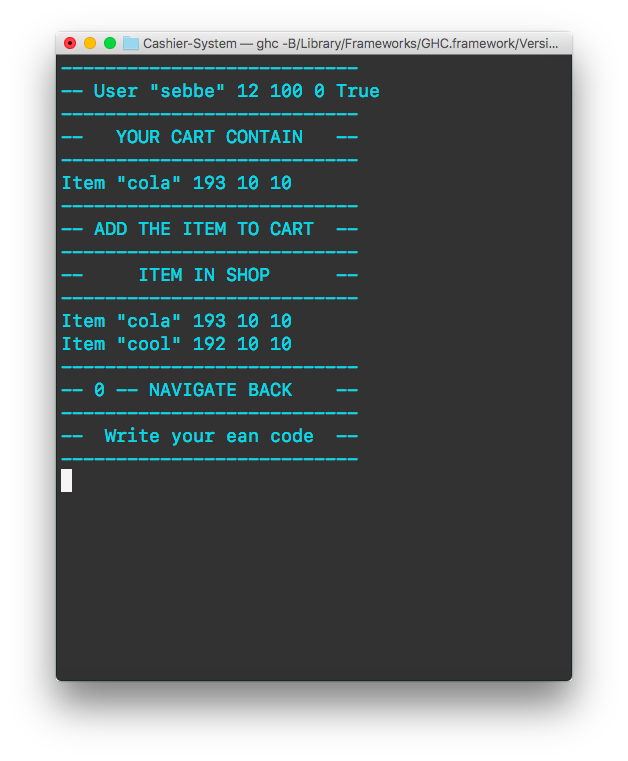
\includegraphics[width=250px]{interface3.png}
  \caption{adding and removing item}
\end{figure}
\\
\newpage
The interface has now updated. The 3rd section (menu) is now a list with items in the shop. If we want to add the item “cola” we’ll have to scan, or write the ean code for the item in the command line which in this case is 193 and then press enter. If you don’t feel like buying anything we can navigate to the menu by dimply typing in “0” and hit enter.
\\
\begin{figure}[h!]
  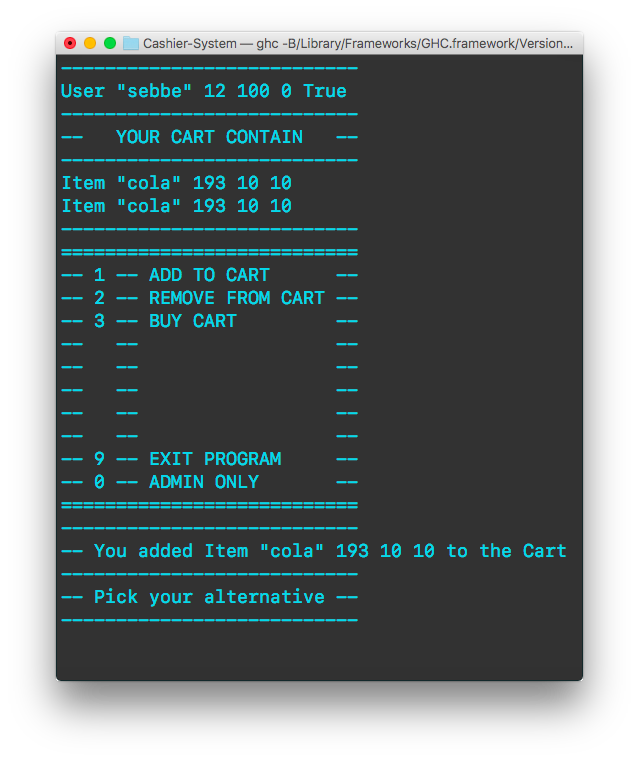
\includegraphics[width=250px]{interface4.png}
  \caption{aftermath adding}
\end{figure}
\\
\newpage
As we can observe we now have a new item in the cart and a new message in the  message section, informing us about our last action.We’re now back where we began shopping and ready to proceed. To remove an item the steps are almost identical but instead of typing in “1” we type in “2” and hit enter.
\\
\begin{figure}[h!]
  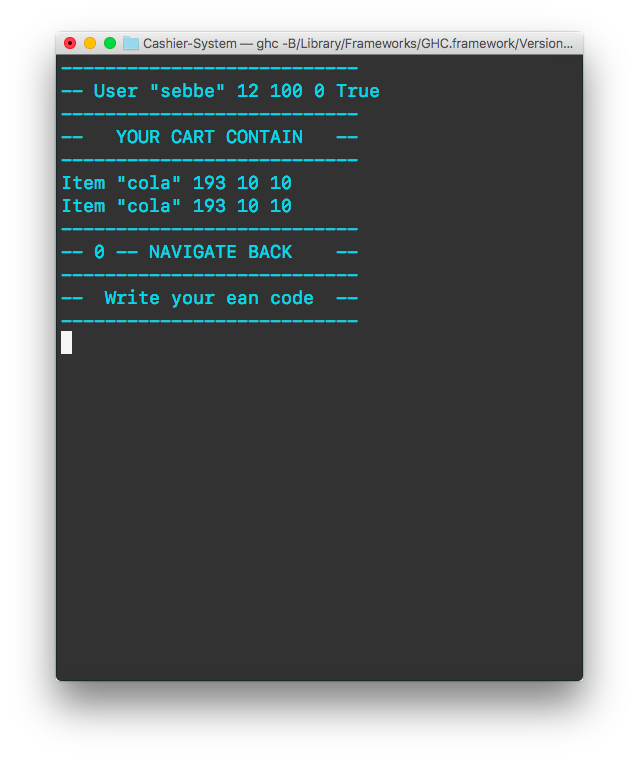
\includegraphics[width=250px]{interface5.png}
  \caption{remove item from cart}
\end{figure}
\\
From here we can remove either of the items in our current cart. To remove the top product “cola”, type in 193 (the ean code) and hit enter. The first cola is now removed and we’re back to only having one item in the cart.\newpage
\subsubsection{Buying a cart}
If you are happy with only having one “cola” and want to purchase the cart, navigate to the menu and type in “3” to buy the cart. The purchase will only granted if you have sufficient funds, You can control that by looking at the second value in the user information where it says 100 (first section). Since we have 100 kr in currency we have no problem in buying the cola for 10 kr. When the purchase is complete the cart is empty, our stored 100 kr is now 90 kr , our spent has gone from 0 to 10 and the message section is informing you that you have bought a cart and it’s content. Observe that there is a limit on how much you buy, since there is a limited stock. If you navigate to the list of purchasable items we can observe how the stock has changed from 10 to 9. Now you have a complete user guide for a customer. However, there are many functions that only is available for an administrator. The following chapter covers all steps required to be a full fledged business system administrator.\\
\subsection{Admin functions}
In the first section the user holds the name, id, funds, money spent and a boolean. The boolean can either be True or False. Whether it’s True or False depends if the user is an admin or not. In this case you can see that the user is admin. Thus, allowing the user to access all admin functions, if the bool would have been false our access would have been denied. To access the admin functions you type in “0” and hit enter. Once done the message section will tell us if the access was granted or denied.
\\
From here we can modify items, add items, add users and modify users. Let’s begin with “User fixes” by pressing “1” [enter]
\\
\begin{figure}[h!]
  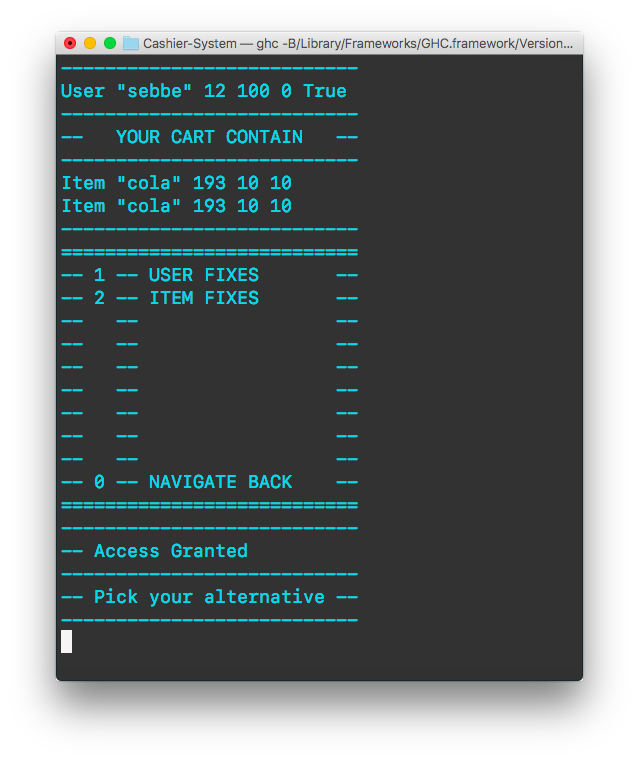
\includegraphics[width=250px]{interface6.png}
  \caption{Admin functions}
\end{figure}
\\
\subsubsection{User fixes}
Your Business System should now present the following information.
\\
\begin{figure}[h!]
  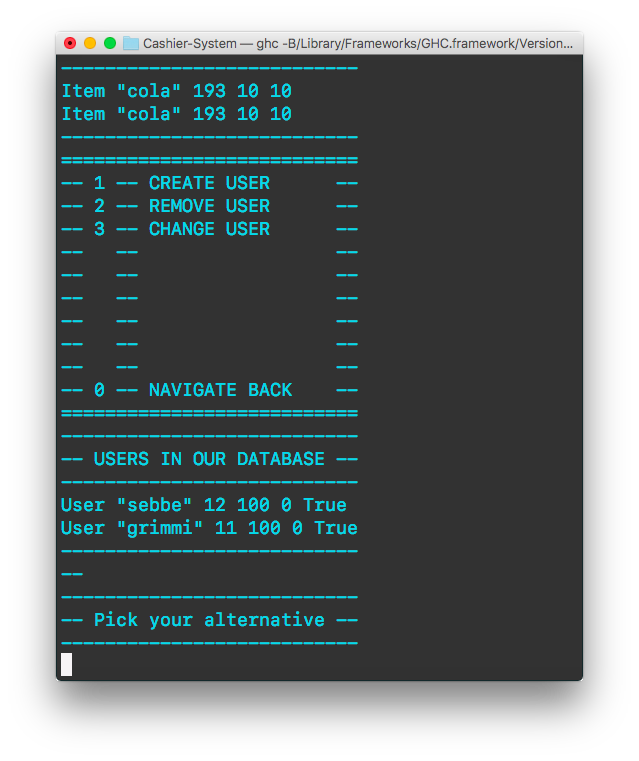
\includegraphics[width=250px]{interface7.png}
  \caption{User fixes}
\end{figure}
\\
Here we can see the current users in our database we also get four new alternatives we can either create a user, remove a user, change user or change the wallet. We will work from the top down explaining the different functions.
\newpage
To create a new user, navigate as usual by pressing “1” and hit [enter]. Follow the instructions the terminal is giving. First type in the name of the user and hit [enter], now write the id of the user which is a positive integer and hit [enter]. Next, type in how much money you want the account to withhold. the input must be an positive integer, then hit [enter]. The last thing you need to put in is the admin status, which can either be True or False with a capital first letter, then hit [enter]. If everything has been applied correctly there is now a new user in the database and you have created a new account.\\\\
To remove a user, type in “2” and hit [enter]. Once done you do as the terminal says. ”Write id of the user you want to remove”,  then hit [enter]. The message section is now informing you that a user has been removed and there is one less user in the database.\\\\
To change a user, press “3” and hit [enter]. Follow the instructions from the terminal and pick a suitable id for the user you want to change. if the id is valid you will get five more options. you can either change the user name, id, fill the wallet, reduce the wallet or clear the wallet.
\\
\begin{figure}[h!]
  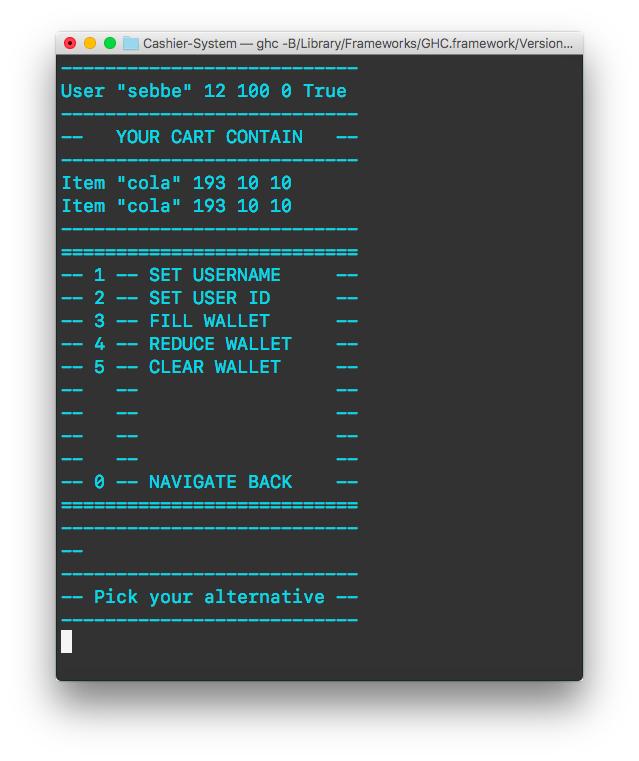
\includegraphics[width=250px]{interface8.png}
  \caption{Edit user}
\end{figure}
\\
\newpage
To change the username, press “1” and hit [enter]. Type in the new username, then press [enter].
To change the user ID, press “2” and hit [enter],  then type in a new user ID. Note that the ID has to be positive integers.\\
To fill the wallet, press “3” and hit [enter], now type in the amount you want the wallet to be filled with, its has to be positive.\\
To reduce the amount of money in the wallet, press “4” and hit [enter], now type in a positive value of how much you want to reduce the wallet with.\\
To remove all available money from the wallet, Press “5” and [enter].  All the funds will be removed.\\
You can always follow what you have changed, if you are changing your own profile you can see in the user section when the changes occurs. If it is not your account you’re changing the message section will update what changes has been done.\\\\
\subsubsection{Item fixes}
By navigating back to the admin only page, we can again choose between user fixes or item fixes. This time pick item fixes by typing “2” and hit [enter]. Here you can create new items, remove items and change items.
\\
\begin{figure}[h!]
  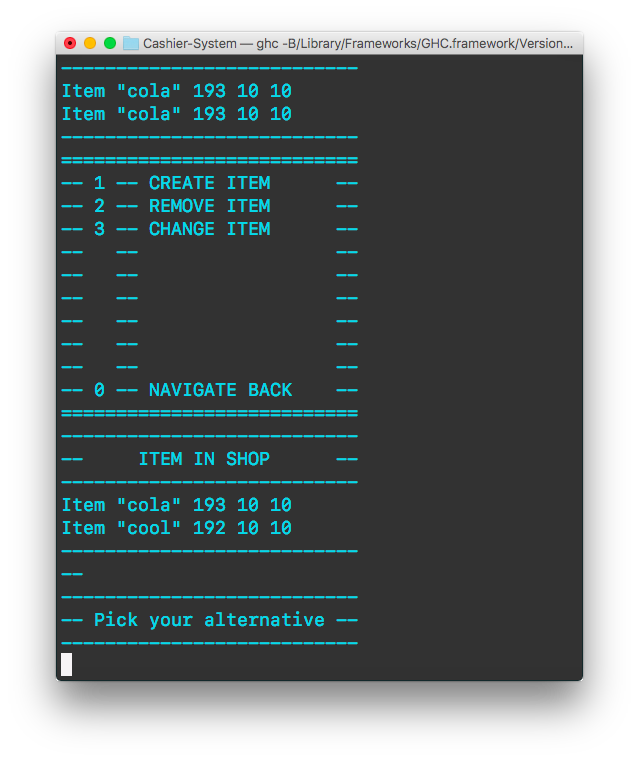
\includegraphics[width=250px]{interface9.png}
  \caption{Item fixes}
\end{figure}
\\
\newpage
To create an item we type in “1” and follow the instructions that the terminal gives. First off, enter the name of the item and hit [enter]. Next type in the EAN code and hit [enter]. Now enter the price of the item and hit [enter].Last, enter the stock value of the item. The message section is now informing you that a new item has been created and a new item is visible in the shop.\\\\
To remove an item we type in “2” and hit [enter]. Type in the EAN code for the item we want to remove and hit [enter] again.\\\\
To edit an item, begin by typing in “3” and press [enter], then type in the ean code for the item you want to change. Once done you are now able to edit the item chosen.\\
To change the name press “1” and hit enter, now type in a suitable name for the item and press enter.\\
To change the EAN code, type in “2” and hit [enter], now enter a valid EAN code for the item.
To change the price type in “3” and hit [enter], now enter a suitable price for the item.\\
To add stock type in “4” and hit [enter], now type in how much stock should be added for the item.
To remove stock type in “5” and hit [enter], now type in how much stock you want to remove, the stock is not allowed to go below zero.\\
To replace stock type in “6” and hit [enter],  now type in the amount you want the item to have in stock.\\\\
You should now be able to navigate through the whole business system and operate changes as an admin, or shop products as a Customer. Hopefully the system is self explaining in its preset of available choices and status updates. Good luck, have fun, and shop responsibly!
\newpage
\section{Algorithms}
\subsection{Recursive algorithms}
The business system is built on various functions and mathematical algorithms. One of the most common function types applied is recursive algorithms, or recursion. We specify recursive algorithms as a function that takes its own values to generate an infinite loop until the desired answer is reached. To apply the recursion it is important that the programmer specifies grid values in which the algorithm should operate, and end cases onto the recursion returns values. (http:\\www.dictionary.com/browse/recursion)Retrieved: 2017-02-20 \\
\begin{lstlisting}
grabWithId.
grabWithId :: Id -> Database a -> a
grabWithId i [] = error "not in our database"
grabWithId i (x:xs)
  | i == (snd x) = fst x
  | otherwise = grabWithId i xs
\end{lstlisting}
grabWithId initially takes an ID from and the database it’s supposed to search. Further it makes fault values if the database is empty. What the algorithm then does is using recursion to walk through the list of users searching for a match to the identity code. for each comparison made it either goes to the next value, or gets a match and returns the User holding the right identification. If the list is compared completely without result it interprets the list as empty and returns an error. namely "not in our database".\\
\\
This way we can see a typical recursion example where the algorithm uses itself to walk through the information in order to return a desired value or result.
To understand Recursions further, please read attached pre- and post conditions on applied functions in attached file.\\
\subsection{Pattern matching}
in our business system we are applying pattern matching functions. The specification of the function type defines by giving the computer a given sequence, or pattern in which it matches the functions definitions. By giving the computer a parameter, or matching data type to what we want to achieve, it replaces the original value or adds a new one.(https:\\www.haskell.org/tutorial/patterns.html)
To exemplify this we have attached an example out of our own code of a pattern matching function.
\begin{lstlisting}
setName :: Name -> Item -> Item
setName x (Item name ean price stock) = Item x ean price stock
\end{lstlisting}
setName is hands on in its command as it takes an input that will replace the x in the fitting pattern of an item. for example in setName it takes a String and an Item, onto it wants the user to clarify what String of characters it wants to declare as the items name.
In application setName “coca-Pepsi” returns an item with the name “coca-Pepsi” with attatched specifications such as the data type Item is supposed to hold. eg. (Name, Ean, Price, Stock). To understand Pattern matching further, please read pre- and post conditions on applied functions in attached file.
\newpage
\section{Tests \& Debugging}
We have applied automated tests by the module HUnit.\\
Hunit is a testing framework for the programming language Haskell. The methodology of the framework is to be able to easily create, and edit tests that are automatically conducted by the program in order find errors or problems with the code faster and intelligible (https:\\hackage.haskell.org/package/HUnit)
\\
Please read further in attached file for all HUnit tests.
\\
The ambition to this project is to have at least one automated test for each function and getting 0 errors, or faults in the program. However, we believe that this might be insufficient to account for complete functionality of the program.
\newpage
\section{Shortcomings of the program}
\subsection{Test cases}
Due to the time frame of the project we have not satisfied the complete need for test cases throughout the whole system. However, we have conducted some tests. We are aware that they are not covering all bases. This implies that hidden faults are possible to interrupt the functionality of the system. However, so far we have not encountered any non-expected errors in the program. If more time was offered we would have conducted more tests on the system in order to cover the complete functionality of all functions.
\subsection{Run time cost}
The business system is currently handling the search and action based functions in an non-effective way. This is because the run-time cost of functions generally are T:(n) = n, which can be defined as linear run time cost . This means that most actions and recursive algorithms are processed one unit or value at a time. Thus, making the system slower than necessary. However, since haskell is generally processing values fast and the database is currently handling small amounts of information, it is not recognisable at this development state and is therefore not a priority in the project.
\subsection{Advancement time frame}
As many projects, This business system project was initially striving to obtain a complete high quality business register program with a highly scaleable framework. As we completed the base-platform for the system we discovered that only a few additional functions was able to be done in time and we decided to focus more on the quality of the surrounding project issues other than expanding the systems functionality. Thus, the goal was obtained to complete a scaleable project. However we believe that more time would benefit the projects usability and quality.
\subsection{Usability graphical framework}
We are all agreeing that the system would benefit from a more graphical interface. If the system could access a more usable interface directed to the common non-technical user the quality of the program would increase significantly.
\end{document}
